\section{Sistemas de reconhecimento de caracteres}
	
	Segundo \cite{silva2003reconhecimento}, os sistemas de reconhecimento ótico de caracteres são sistemas desenvolvidos para, de certa forma, reproduzir a capacidade humana de ler textos.

	\subsection{Origens e Evolução}
	
		\cite{man1986pattern} disse que as origens da tentativa de sumular a leitura humana datam de 1870, quando foi inventado por Carey, o scanner de retina. A partir da evolução dos dispositivos capazes de captar e traduzir imagens em sinais que podiam ser medidos, novos horizontes foram descobertos. Entretanto, a primeira tentativa bem sucedida de reconhecimento de caracteres foi realizada somente em 1990 pelo cientista russo Tyutin, que desenvolveu um sistema que visava o auxílio de deficientes visuais.
	
		Alguns dos motivos do desenvolvimento de um sistema de reconhecimento de caracteres são:
		
		\begin{itemize}
			\item Aquisição de dados numéricos comerciais;
			\item Compactação de dados;
			\item Leitura automática de formulários;
			\item Identificação de endereçamento postal;
			\item Reconhecimento de cheques bancários;
			\item Sistemas de aquisição de textos para a tradução automática;
			\item Interface homem x máquina mais natural e sem necessidade de recodificação dos dados (sujeitos a um menor número de erros, pois não é necessário redigitar os textos, introduzindo novos erros);
			\item Auxílio a deficientes visuais, na leitura de textos (tradução e impressão automática em braile)
		\end{itemize}

	\subsection{Tipos de Sistemas de Reconhecimento de Caracteres}
		
		Os sistemas de reconhecimento de caracteres podem ser desenvolvidos utilizando-se diferentes procedimentos tanto de aquisição de dados como de processamento de informações além de serem orientados para diferentes tipos de aplicações.
	
		Podem ser classificados primeiramente quanto ao tipo de mecanismo utilizado na aquisição dos textos a serem reconhecidos. Nesta categoria, encontram-se os sistemas magnéticos, sistemas mecânicos e sistemas óticos.
	
		Dentro dos sistemas OCR, são encontradas duas classes importantes, aqueles que são baseados no processamento sequencial das informações e os baseados no processamento paralelo. Existem três categorias princiapais: sistema de reconhecimento online, sistema de reconhecimento de caracteres isolados e sistema de reconhecimento de escrito cursiva.
	
	\begin{figure}[!htb]
		\centering
		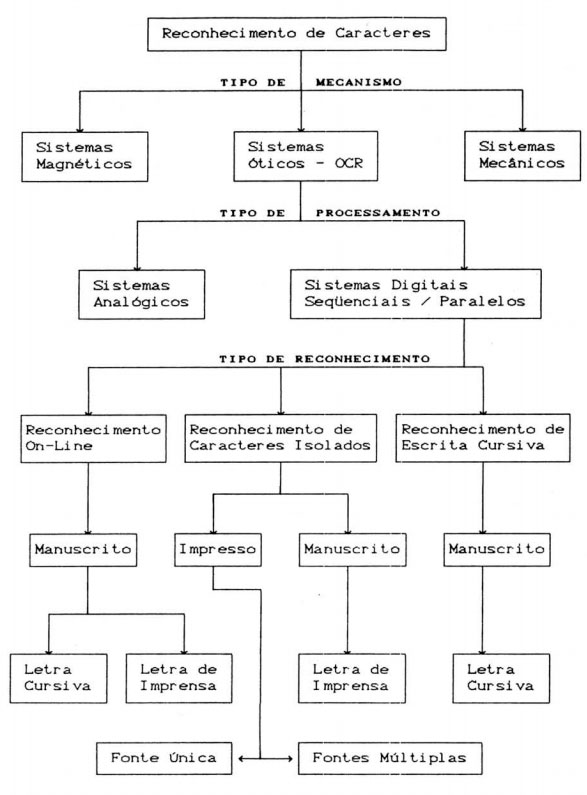
\includegraphics[scale=0.4]{img/organograma-tipos.jpg}
		\caption{Organograma}
		\label{Organograma}
	\end{figure}
	
	\subsection{Descrição dos Sistemas OCR}
		
		Existem diferentes etapas de processamento das informações visando o reconhecimento de textos por um sistema OCR. Estas etapas se estendem desde a captura da imagem do texto até a obtenção final de uma identificação deste. Em um sistema de COR não se deve considerar apenas a parte referente às técnicas empregadas na resolução do problema de classificação, mas um item de extrema importância é a medicação e avaliação dos resultados obtidos por estes.
		
		\subsubsection{Etapas de Processamento}
			
			Em geral, os sistemas de OCR possuem implementadas as seguintes funções: aquisição da imagem do texto, tratamento da imagem, localização e separação dos caracteres, pré-processamento dos padrões, extração de atributos, reconhecimento/classificação dos padrões e pós-processamento.
		
		\begin{figure}[!htb]
			\centering
			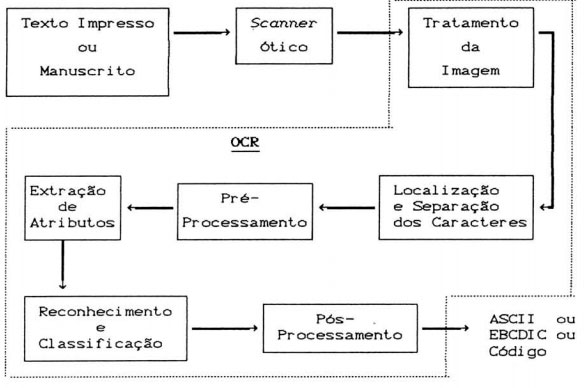
\includegraphics[scale=0.5]{img/etapas-de-processamento.jpg}
			\caption{Etapas do processo de reconhecimento}
			\label{Etapas do processo de reconhecimento}
		\end{figure}
		
		Para a separação dos caracteres, o algoritmo tem que levar em consideração diversos fatores, entre eles: o espaçamento entre caracteres e tamanho do caractere (fixo ou variável), a utilização de uma grade auxiliar (no caso de formulários com espaçamento bem definidos), e o tipo de texto a ser reconhecido, onde podem haver caracteres que se tocam ou caracteres com descontinuidade (características muito importante para módulos de segmentação). Esta etapa de processamento é até hoje uma das etapas mais críticas, sendo um problema ainda não completamente solucionado.
		
		Após terem sido isolados os caracteres, e preferencialmente, com a realização de um ajuste de tamanho e posição pré-definidos, pode-se então realizar uma etapa de extração de atributos. Esta etapada é opcional e dependerá exclusivamente do tipo de técnica empregada no reconhecimento e classificação dos padrões.
		
		\subsubsection{Técnicas de Reconhecimento}
			
			Existem diferentes técnicas empregadas no reconhecimento de padrões, mas estas podem ser classificadas em três grandes categorias, técnicas baseadas em:
			
			\begin{description}
				\item \textbf{Atributos globais}: Nesta categoria, os atributos (features) são extraídos de cada ponto interior ao retângulo que circunscreve a matriz do caractere a qual também pode ser denominado de \textit{frame}. Os atributos empregados não refletem nenhuma propriedade local, geométrica ou topológica do próprio traçado. Algumas dessas técnicas foram desenvolvidas originalmente para reconhecer apenas caracteres impressos.
				\item \textbf{Distribuição de pontos}: É uma outra forma de reduzir a dimensionalidade dos conjuntos de atributos, onde estes são derivados a partir das distribuições estatísticas dos pontos. Diferentes tipos de distribuições tem sido utilizadas correspondendo a diferentes técnicas de reconhecimento.
				\item \textbf{Atributos geométricos e topológicos}: Esta técnica é baseada na extração de atributos que descrevem a geometria ou topologia de interesse no traçado do caractere. Estes atributos podem representar propriedades locais. Esta é de longe a mais popular técnica estudada pelos pesquisadores. 
			\end{description}
	
		\subsubsection{Avaliação do Reconheimento}
			
			Uma das formas de realizar a avaliação destes sistemas foi através da criação de bancos de dados padrões para análise de desempenho, contendo amostras variadas de pares a serem reconhecidos par um novo algoritmo submetido a avaliação de alguns destes bancos de amostras de pares de caracteres se tornaram muito difundidos e utilizados na avaliação de diferentes sistemas. Dois destes bancos de dados muito conhecidos são: o de Highleyman e o de Munson. Estes bancos de dados estão disponíveis junto ao IEEE e fornecem um conjunto de caracteres manuscritos em letra de impressora. Os dados de Munson possuem 12760 amostras de 46 tipos diferentes de caracteres, com uma resolução de 24 x 24 pixels, e os dados de Highleyman possuem 1800 amostras de letras e 500 de numerais, com um total de 36 tipos diferentes de caracteres, com uma resolução de 12 x 12 pixels. Esta resolução (12x12) infelizmente não é a mais adequada, uma vez que para a reconhecimento de caracteres manuscritos é aconselhada uma matriz com dimensões em torno de 20 x 25 pixels. O maior problema referente a tais bancos de dados 6 a divulgação de sua existência e as formas de acesso aos mesmos. Infelizmente, para a realização deste trabalho não foi possível a utilização destas bases de dados de pares de caracteres, devido primeiramente ao fato de serem orientados a sistemas de reconhecimento de caracteres manuscritos e, em segundo, porque não foi possível até o momento ter acesso a eles.
			
			Os principais parâmetros a serem tomados como referenda são os índices de avaliação de desempenho de sistemas de OCR. Estes índices consistem de três indicadores: taxa de caracteres reconhecidos corretamente, taxa de caracteres substituídos (classificações incorretas) e taxa de rejeição (caracteres não identificados).

	\subsection{Redes Neurais}
		
		As redes neurais foram desenvolvidas a partir de uma tentativa de criar um modelo que descrevesse a estrutura e o funcionamento dos neurônios do cérebro humano. Os modelos de redes neurais buscam definir novos computadores ou novos modelos de processamento de dados. Estes devem apresentar um comportamento baseado em modelos neurobiológicos ao invés de modelos baseados em "circuitos de silício" (portas lógicas, circuitos combinacionais, biestáveis, etc).
		
		\subsubsection{Características e Aplicações das Redes Neurais}
		
			As redes neurais possuem a característica de serem muito apropriadas ao reconhecimento de padrões. Como já foi visto, as redes neurais podem sofrer um aprendizado, modificando seu comportamento frente a um conjunto de estímulos de entrada (padrão de entrada). Portanto, a rede pode aprender a dar uma resposta específica Para um determinado conjunto de estímulos fornecidos. Isto será obtido através da alteração dos pesos de atuação das entradas. 124 Logo as redes neurais são muito adequadas para reconhecimento e classificação de pares, pais podem se adaptar para responder a um padrão específico. As redes neurais possuem também uma alta velocidade de processamento, devido ao seu maciço paralelismo interno, possibilitando o desenvolvimento de certos tipos de aplicações complexas que necessitam operar em tempo real. Devido às características inerentes às redes neurais, estas podem realizar alguns tipos de tarefas que não são executadas de uma forma satisfatória em sistemas computacionais tradicionais, mas que para a ser humano são tarefas triviais. Elas possuem a característica de se adequar perfeitamente às seguintes aplicações:
			
			\begin{itemize}
				\item Reconhecimento e síntese contínua da fala;
				\item Reconhecimento visual de padrões e padrões em geral 
				\item Reconhecimento e classificação de imagens como, por exemplo: textos, assinaturas, impressões digitais, objetos, etc;
				\item Processamento adaptativo de sinais e eliminação de rut dos;
				\item Aplicações onde as dados fornecidos são incompletos e os resultados produzidos são aproximados
			\end{itemize}